\section{Encoder-Decoder}
\label{encoderDec}
\subsection{Généralités}
Les \textit{Encoder-Decoder} sont une famille de réseaux dont l'appellation provient du \textit{traitement du signal}. Un réseau \textit{Encoder-Decoder} se compose de deux parties: la partie Encoder et la partie Decoder. Ces deux parties sont formées par deux réseaux indépendants.\\

\noindent L'objectif de l'Encoder est de représenter la donnée d'entrée (définie dans un espace $\mathcal{X}$) dans un espace $\mathcal{Z}$ souvent de dimension inférieure. La donnée obtenue s'appelle \textit{vecteur de contexte} (context vector ou code). Dans le cas où la dimension de l'espace de sortie est inférieure à celle de l'espace d'entrée, on dit que la représentation de l'entrée est \textit{compressée}. \\

\noindent Le Decoder est le complémentaire de l'Encoder. Il exploite la projection de l'Encoder afin de créer une nouvelle projection dans un autre espace souhaité. Il n'y a aucune obligation à conserver le même espace que celle de la donnée d'entrée ou du vecteur de contexte. La non-obligation de conservation de l'espace permet de rendre l'application de ce type d'architecture très diversifiée, notamment dans le cadre du nettoyage/réduction des données (pré-processing), la traduction multi-langue et la génération de données artificielles.\\

\noindent Ainsi, nous pouvons résumer l'action d'un Encoder-Decoder par:
$$\phi: \ \stackrel{\mathcal{R}^X}{x} \stackrel{\rightarrow}{\longrightarrow} \stackrel{\mathcal{R}^Z}{\phi(x)}$$
$$\varphi: \ \stackrel{\mathcal{R}^Z}{z} \stackrel{\rightarrow}{\longrightarrow} \stackrel{\mathcal{R}^Y}{\varphi(z)}$$
$$ED: \ \stackrel{\mathcal{R}^X}{x} \stackrel{\rightarrow}{\longrightarrow} \stackrel{\mathcal{R}^Y}{\varphi(\phi(x))}$$

\noindent Avec $\phi$, la fonction de l'Encoder et $\varphi$, celle du Decoder.

\subsection{Autoencoder}
Un \textit{Autoencoder}\cite{autoencoder} est un cas particulier d'architecture Encoder-Decoder. Il est caractérisé par un espace de projection du Decoder identique à celui de la donnée d'entrée et l'objectif est de "retrouver" la donnée d'entrée. Ainsi, l'action d'un Autoencoder peut être définie par:
$$\phi: \ \stackrel{\mathcal{R}^X}{x} \stackrel{\rightarrow}{\longrightarrow} \stackrel{\mathcal{R}^Z}{\phi(x)}$$
$$\varphi: \ \stackrel{\mathcal{R}^Z}{z} \stackrel{\rightarrow}{\longrightarrow} \stackrel{\mathcal{R}^X}{\varphi(z)}$$
$$ED: \ \stackrel{\mathcal{R}^X}{x} \stackrel{\rightarrow}{\longrightarrow} \stackrel{\mathcal{R}^X}{\varphi(\phi(x))} \rightarrow x$$

\noindent L'Autoencoder est composé de structures comparables à un modèle Feed-Forward (Full-Connected) ou convolutif. Son apprentissage est donc possible avec une approche classique. Pour cela, la rétropropagation du gradient et les fonctions de coût standards sont employées. Ainsi, pour une donnée d'entrée binaire x de dimension n, nous utilisons la \textit{Binary Cross-Entropy}:
$$\mathcal{L}(\theta)= -\sum_{i=1}^n \left[x_i \log(\hat{x}_i) + (1-x_i) \log(1-\hat{x})\right]$$

\noindent Dans le cas d'une entrée x à valeur réelle dans $\mathcal{R}^n$, nous préfèrerons la \textit{Mean squared error} (MSE):
$$\mathcal{L}(\theta)= \frac{1}{n}\sum_{i=1}^n (\hat{x_k}-x_k)^2$$
\noindent Du fait que l'objectif est d'obtenir à nouveau la donnée d'entrée, la labellisation de la donnée d'apprentissage est inutile, ce qui fait d'un Autoencoder, une méthode d'apprentissage \textit{non supervisé}.\\

\noindent Un Autoencoder peut avoir une ou plusieurs couche cachées. Dans le cas d'accumulation de couches cachées, nous parlerons de \textit{Deep Autoencoder}. Les Deep Autoencoder favorisent l'utilisation de fonction d'activation non linéaire, l'exploitation de couche de convolution au détriment des couches Full-Connected et ont un grand pouvoir explicatif. Le risque d'overfitting est donc plus important et demande une attention particulière.\\

\noindent L'approche standard de l'Autoencoder est essentiellement utilisée dans le cadre d'une réduction de dimension\footnote{Ce modèle est capable d'approximer les résultats d'une ACP linéaire et non linéaire par exemple}. Elle est donc utile pour réaliser une compression de donnée ou du pré-processing de données. Ils sont aussi utilisés dans le cadre d'une recherche de complétion de données en présence de données incomplètes ou partiellement corrompues.

\subsubsection{Autoencoder Undercomplete}
L'\textit{Autoencoder Undercomplete} est souvent associé à l'architecture de base d'un Autoencoder. L'idée derrière cette architecture est de réaliser une projection de la donnée d'entrée sur un espace de dimension plus \textbf{faible}. Ainsi, l'Encoder est défini par:
$$\phi: \ \stackrel{\mathcal{R}^X}{x} \stackrel{\rightarrow}{\longrightarrow} \stackrel{\mathcal{R}^Z}{\phi(x)} \ avec \ Z \ll X$$

\noindent La projection sur un espace de plus petite dimension force l'Autoencoder à extraire l'information importante des données d'entrée. Si la dimension de l'espace de projection est identique à celle de l'espace de la donnée d'entrée, le modèle aura tendance à apprendre la fonction \textit{identité}, ce qui empêchera l'extraction d'information des données. Cette particularité rendra donc inutile l'Encoder et de ce fait, le Decoder car le vecteur de contexte tendra à être équivalent à la donnée d'entrée. Une représentation d'un Autoencoder est visible sur la Figure \ref{autoencoder}.

\begin{figure}
    \centering
    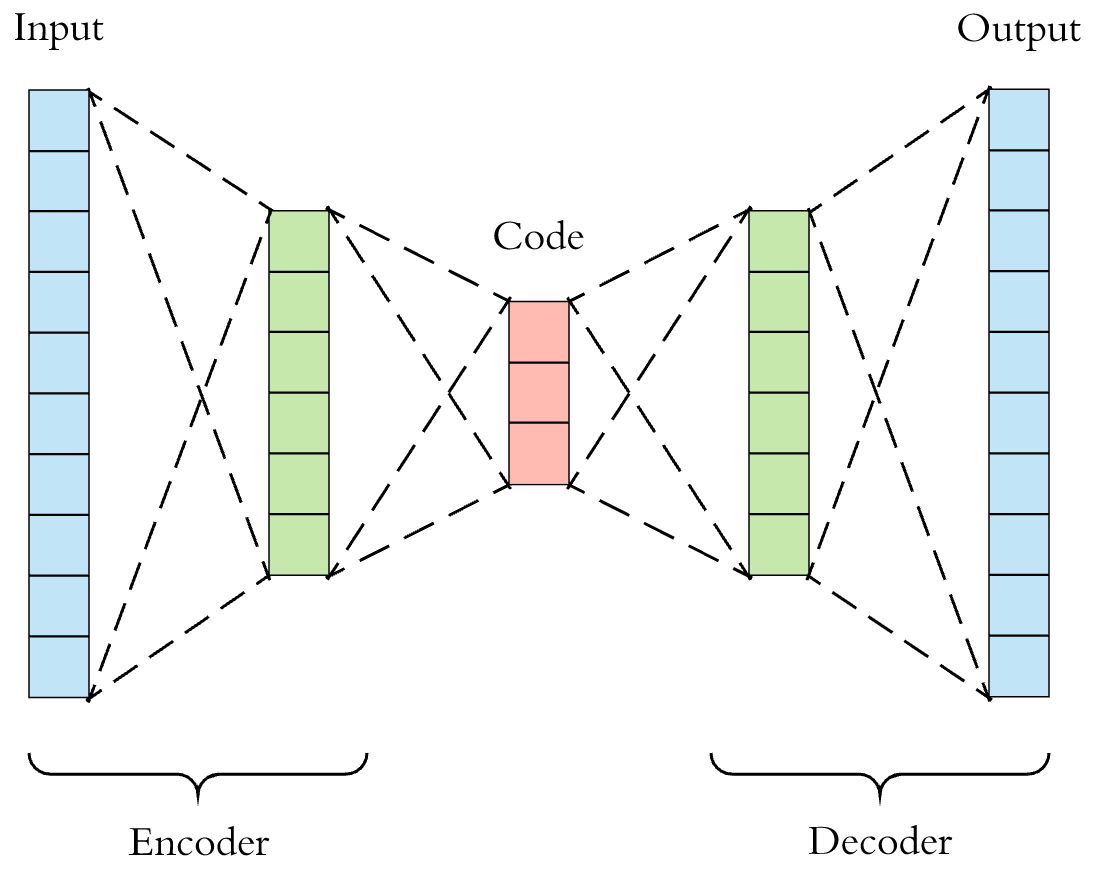
\includegraphics[scale=0.2]{./tex/encoder-decoder-network/autoencoder.png}
    \caption{Architecture d'un Autoencoder}
    \label{autoencoder}
\end{figure}

\subsubsection{Autoencoder Régularisé ou Overcomplete}
Un \textit{Autoencoder Overcomplete} s'émancipe de la dimension du vecteur de contexte et propose de réaliser une projection sur un espace de dimension identique voire supérieure. Afin de lutter contre le risque de création d'une représentation \textit{identité}, cette architecture \textit{régularise} la fonction de coût pour pousser le modèle à extraire des propriétés des données au lieu d'une simple représentation de l'identité de la donnée d'entrée. Cette approche tend à être plus robuste et plus efficace que la méthode Undercomplete.\\

\noindent Il existe différentes régularisations possibles afin de réaliser ce type d'Autoencoder. Ces méthodes peuvent être associées et sont encore un sujet de recherche actuel.

\paragraph{Denoising Autoencoder}
Au lieu d'analyser la donnée d'entrée intègre, un \textit{Denoising Autoencoder}\cite{denoisingauto} exploite la donnée d'entrée \textit{bruitée}. Ce réseau doit donc apprendre à débruiter au lieu d'uniquement \textit{copier} l'entrée.\\

\noindent Il existe différente méthode pour bruiter les données (application d'un bruit gaussien, filtre quelconque, etc... ). En pratique, l'approche la plus populaire consiste à désactiver aléatoirement des neurones de la couche d'entrée en forçant leurs sorties à 0. Cette méthode est comparable à l'application d'un DropOut sur la couche d'entrée du réseau. Une illustration de ce réseau est visible sur la Figure \ref{denoiseauto}.\\

\begin{figure}
    \centering
    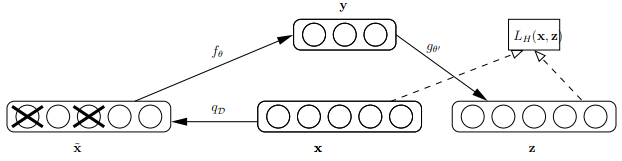
\includegraphics[scale=0.4]{./tex/encoder-decoder-network/denoiseauto.png}
    \caption{Architecture d'un Denoising Autoencoder}
    \label{denoiseauto}
\end{figure}

\noindent \textbf{Important} Lors du calcul de la fonction de coût, la comparaison est réalisée avec la donnée intègre et non la donnée bruitée ! Comparer à la donnée bruitée reviendrait à réaliser un Autoencoder qui apprendrait à représenter les données bruitées et non intègres.\\

\noindent Un \textit{Denoising Autoencoder} est donc défini par:
$$Noise: \ \stackrel{\mathcal{R}^X}{x} \stackrel{\rightarrow}{\longrightarrow} \stackrel{\mathcal{R}^X}{Noise(x)}$$
$$\phi_{Noise}: \ \stackrel{\mathcal{R}^X}{x} \stackrel{\rightarrow}{\longrightarrow} \stackrel{\mathcal{R}^Z}{\phi(x)}$$
$$\varphi: \ \stackrel{\mathcal{R}^Z}{z} \stackrel{\rightarrow}{\longrightarrow} \stackrel{\mathcal{R}^X}{\varphi(z)}$$
$$ED: \ \stackrel{\mathcal{R}^X}{x} \stackrel{\rightarrow}{\longrightarrow} \stackrel{\mathcal{R}^X}{\varphi(\phi(Noise(x)))\rightarrow x}$$

\noindent Cette architecture peut être utilisée pour créer un \textit{débruiteur}. En effet, dans la méthode standard, la donnée intègre est corrompue par une architecture particulière du réseau ou l'ajout d'un bruit artificiel en amont. Nous créons donc, en interne, un jeu de données composé d'entité $[donnee_{integre}, donnee_{bruitee}]$. Le réseau devient donc robuste à corriger les effets du bruit introduit dans ces données. Neanmoins, la correction du bruit est, dans cette configuration, peu utile d'un point de vue métier. Une autre approche serait de réaliser un apprentissage \textit{supervisé} où les données d'entraînement sont issues d'un jeu de données corrompues par un bruit spécifique. L'entraînement sur ce jeu de données permettra ainsi d'obtenir un modèle apte à débruiter un message utile soumis au bruit présent dans les données d'entraînement. Ce modèle obtenu aura donc une plus-value métier car capable de réaliser un débruitage \textit{utile}. On peut voir une application directe dans le cadre des télécoms.

\paragraph{Sparse Autoencoder}
Le \textit{Sparse Autoencoder}\cite{sparseauto} cherche à rendre son architecture éparse\footnote{On parle de \textit{sparsity constraint}}, i.e éviter que l'intégralité des neurones soit forcée d'être stimulée à chaque donnée d'entrée. Cette approche tend à rendre les neurones plus spécialisés en limitant leurs degrés de liberté qui pourraient nuire à la qualité du neurone si les données sont significativement différentes. L'objectif est donc de rendre un neurone sensible à une stimulation spécifique et non l'ensemble des stimulation qu'il reçoit. Ainsi, un neurone doit être inactif la majorité du temps. Cette caractéristique est très importante en présence de données significativement distinctes tels que des jeux de données multi-classes.\\

\noindent Afin de réguler l'activité des neurones, deux approches sont essentiellement employées: La régularisation par la Divergence de Kullback-Leibler ou la k-Sparse constraint.\\

\begin{itemize}
    \item \textbf{KL-divergence}: La régularisation par la KL-divergence modifie la fonction de coût en rajoutant un facteur correspondant à la divergence de Kullback-Leibler.\\

    Supposons un neurone $i$ appartenant à une couche cachée et $a_i$, son activation. On notera $a_i(x_j)$ l'activation du neurone i selon la donnée d'entrée $x_j$. On peut donc définir la valeur moyenne d'activation du neurone i sur un jeu de données de m éléments par: $\hat\rho_j = \frac{1}{m} \sum_{j=1}^m \left[ a_i(x_j) \right]$. \\

    Nous voulons que $\hat\rho_j=\rho$ où $\rho$ est le paramètre déterminant le degrés de dispersion du réseau. $\rho$ doit être faible (supposons 0.05). Cela signifie que nous souhaitons que la moyenne d'activation tende vers 0.05. Ainsi, cette condition impose que le neurone soit constamment éteint (activation proche de 0) en dehors de phase d'activation ponctuelle où la valeur tendra vers 1. Cette condition suppose une activation dans $[0,1]$ telle que l'activation via une sigmoide\footnote{Il est possible de considérer d'autre fonction telle que tanh en modifiant les conditions d'excitation/repos du neurone. Il est cependant nécessaire de considérer des fonctions qui présentent des bornes asymptotiques vers les infinis.} par exemple.\\

    Le statut d'un neurone peut être simplifié par une approximation binaire: allumé ou éteint. Ainsi, on peut considérer l'état d'un neurone comme un problème explicable par la loi de Bernouilli. La divergence de Kullback-Leibler permet de calculer la différence entre deux distributions. Ainsi, il est possible de déterminer la différence entre la distribution des activations du neurone réel (variable aléatoire de Bernouilli de moyenne $\hat\rho_j$) et la distribution idéale souhaitée (variable aléatoire de Bernouilli de moyenne $\rho_j$). Le calcul de la différence est défini par:
    $$KL(\rho || \hat\rho_j) = \rho \log \frac{\rho}{\hat\rho_j} + (1-\rho) \log \frac{1-\rho}{1-\hat\rho_j}$$

    $KL(\rho || \hat\rho_j)$ est égale à 0 en cas d'égalité des distributions et augmente lorsque les distributions se différencient. Son action a donc le même comportement qu'une régularisation classique telle que $\mathcal{L}_2$ par exemple. La fonction de coût est donc définie par:
    $$\mathcal{L}(\theta)_{sparse} = \mathcal{L}(\theta) + \beta \sum_{j=1}^{s_2} {\rm KL}(\rho || \hat\rho_j)$$

    \noindent On suppose qu'il y a $s_2$ neurones dans les couches cachées. $\beta$ est un coefficient qui contrôle l'importance donnée à la condition de dispersion du réseau.

    \item \textbf{k-Sparse constraint}\cite{ksparseauto}: Un k-Sparse Autoencoder réalise une action comparable à un DropOut/DropConnect. En effet, l'approche proposée par ce modèle consiste à ne considérer que les k plus grandes valeurs d'activation d'une couche cachée (généralisable à l'ensemble des couches cachées indépendamment les unes des autres) et à mettre à 0, toutes les autres. La rétropropagation du gradient n'est effective que sur les neurones activés. Lors de l'utilisation du modèle, il faudra exploiter les $\alpha k$ valeurs les plus importantes avec $\alpha \geq 1$. Il a été montré qu'un $\alpha$ supérieur à 1 donne des résultats sensiblement meilleurs\footnote{Sans pour autant exagérer sur sa valeur...}. L'impact de la valeur de k est visible sur la Figure \ref{ksparseauto}.

    \begin{figure}
    \centering
    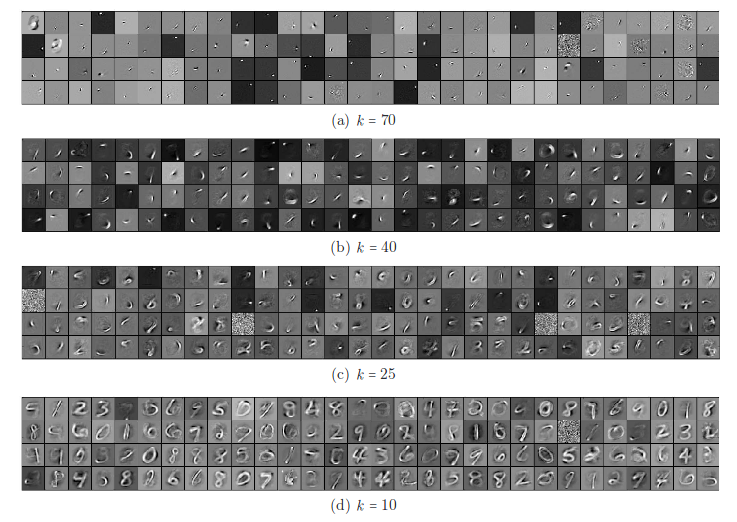
\includegraphics[scale=0.4]{./tex/encoder-decoder-network/ksparse.png}
    \caption{Filtre d'un k-Sparse Autoencoder selon la valeur de k sur le jeu de données MNIST}
    \label{ksparseauto}
\end{figure}
\end{itemize}
\paragraph{Contractive Autoencoders}
Un Contractive Autoencoders \cite{contracauto} repose sur l'idée que le modèle doit être robuste aux changements et éviter des variations importantes dans la représentation du vecteur de contexte (autour des données d'apprentissage). Pour cela, une régularisation par la norme Frobenius de la matrice jacobienne de l'Encoder est utilisée.\\

\noindent La nouvelle fonction de coût est exprimée par:
$$L = \lVert X - \hat{X} \rVert_2^2  + \lambda \lVert J_h(X) \rVert_F^2 $$
$$\lVert J_h(X) \rVert_F^2 = \sum_{ij} \left( \frac{\partial h_j(X)}{\partial X_i} \right)^2$$

\noindent Détaillons le calcul de la régularisation. Supposons une fonction d'activation sigmoïde. Nous avons donc:
\begin{align}
Z_j & = W_i X_i \\[10pt]
h_j & = \phi(Z_j)\\[10pt]
\frac{\partial h_j}{\partial X_i} &= \frac{\partial \phi(Z_j)}{\partial X_i} \\[10pt]
                                 &= \frac{\partial \phi(W_i X_i)}{\partial W_i X_i} \frac{\partial W_i X_i}{\partial X_i} \\[10pt]
                                 &= [\phi(W_i X_i)(1 - \phi(W_i X_i))] \, W_{i} \\[10pt]
                                 &= [h_j(1 - h_j)] \, W_i
\end{align}
On obtient:
\begin{align}
\lVert J_h(X) \rVert_F^2 &= \sum_{ij} \left( \frac{\partial h_j}{\partial X_i} \right)^2 \\[10pt]
                         &= \sum_i \sum_j [h_j(1 - h_j)]^2 (W_{ji}^T)^2 \\[10pt]
                         &= \sum_j [h_j(1 - h_j)]^2 \sum_i (W_{ji}^T)^2
\end{align}

\noindent Ce calcul est très semblable au calcul utilisé durant la retropropagation du gradient. En supposant une couche caché de 20 neurones, alors le problème est déterminé par 20 fonctions définies par un vecteur de gradient chacune d'où l'obtention d'une matrice jacobienne. Il est important de noter que cette régulation exploite une norme de la jacobienne. Cette particularité est intéressante car elle permet d'éviter de devoir définir la matrice diagonale de $[h(1 - h)]^2$. En effet, Ce facteur dépend d'une variable autre que celle de W. Il faut donc associer à chaque dimension de W, l'entité (unique) de $[h(1 - h)]^2$ correspondant, ce qui impose l'exploitation d'une matrice diagonale qui peut être délicate à obtenir.\\

\noindent La régularisation de $\lVert J_h(X) \rVert_F^2$ est uniquement destructrice. Elle punit toute variation associée à l'activation des neurones de l'Encoder. Néanmoins, cette régularisation est compensée par $\lVert X - \hat{X} \rVert_2^2$ qui peut avoir un bon résultat. $\lVert X - \hat{X} \rVert_2^2$ possède un résultat amélioré lorsque la variation demandée au réseau lors d'une mise à jour des poids est bénéfique à l'apprentissage. Au contraire, lors d'une variation sans impact, $\lVert X - \hat{X} \rVert_2^2$ stagne. Dans ce dernier cas, l'impact de la régularisation est trop fort et l'optimisation du réseau ne considérera pas cette possibilité d'évolution. Ainsi, seules les modifications de faible ampleur\footnote{Une variation massive qui produit un gain de performance important peut cependant être accepté. Tout dépend du degrés de variation et du gain de performance associé} autour des données d'apprentissage seront considérées, les autres variations étant \textit{contractées}. Il serait intéressant d'approfondir les problématiques de convergence de cette approche qui présente une faible capacité d'exploration\footnote{Le compromis Exploration/Exploitation est récurrent en apprentissage automatique, notamment en apprentissage par Renforcement}.\\

\noindent Le facteur $\lambda$ est important. En effet, ce paramètre régule l'importance donnée à la régulation. Plus $\lambda$ est élevé, plus les variations seront pénalisées. Un facteur trop important bloquera donc le réseau car aucune variation ne sera jugée suffisamment bénéfique pour compenser la pénalisation de la variation.

\subsection{Variational Autoencoders}
\textbf{Important}: Comprendre ce modèle d'un point de vue théorique nécessite un solide bagage en probabilité (inférence bayesienne). Nous n'approfondirons donc pas l'origine et les démonstrations théoriques de ce modèle.\\

\noindent Le \textit{Variational Autoencoders}(VAE)\cite{varauto1}\cite{varauto2} est l'architecture d'Autoencoder la plus récente. La spécificité de ce modèle est qu'il apprend un modèle de \textbf{variable latente}. Un VAE est donc un \textbf{modèle génératif à conditions}. Contrairement au GAN\footnote{Nous étudierons ce type de modèle par la suite} qui génère des entités aléatoirement, ce type de modèle est capable de générer des entités sous conditions, permettant ainsi de cibler la nature des résultats que nous souhaitons obtenir.\\

\noindent Un Encoder standard réalise une projection d'un vecteur sur $\mathcal{R}^{dim}$. Chaque image d'entraînement est donc clairement définie par un vecteur unique sur $\mathcal{R}^{dim}$. Cet aspect est très problématique lorsque nous désirons un modèle \textbf{génératif} car le Decoder ne peut s'émanciper des données d'apprentissage. En effet, l'espace de projection aura tendance à être très éparse et à présenter différents clusters éloignés les uns des autres et formés par des entités d'apprentissage similaires. Cette discontinuité et les difficultés d'interpolation associées font que le Decoder n'est pas capable de considérer des vecteurs sur $\mathcal{R}^{dim}$ non référencés\footnote{Le Decoder produira un résultat souvent mauvais car il ne "comprendra" pas le vecteur de contexte proposé}. Il n'est donc pas capable d'analyser des vecteurs de contexte inconnus, ce qui est problématique dans le cadre de la génération de données.\\

\noindent Le \textit{Variational Autoencoders} propose une solution à ce problème en introduisant la notion de \textit{variable latente} dans son vecteur de contexte. Au lieu de prédire des valeurs discrètes, l'Encoder va déterminer des paramètres d'une distribution de probabilité, ce qui permet une généralisation efficace. Ainsi, l'Encoder inférera la moyenne et et l'écart-type d'une distribution normale pour chacune des dimensions du vecteur de contexte. L'architecture du réseau est visible sur la Figure \ref{varauto1}. L'Encoder prédit un vecteur moyenne et un vecteur écart-type où chaque dimension de ces deux vecteurs correspondent deux-à-deux aux paramètres d'une distribution normale associée à la dimension concernée du vecteur de contexte. Une explication graphique est montrée par la Figure \ref{varauto2}. Le Decoder recevra donc un vecteur inféré selon les distributions du vecteur de contexte.\\

\noindent Cette configuration présente une problématique majeure. Ne pas régulariser les paramètres favorisera la détermination de moyennes de distribution très éparses et diversifiées (selon les classes de données) avec un écart-type qui aura tendance à être faible. Cet aspect est préjudiciable car nous souhaitons que les données soient les plus proches possibles afin de faciliter les interpolations nécessaires à la création de nouvelles données. Afin de lutter contre ce phénomène, la fonction de coût est régularisée par la divergence de KullBack-Leibler qui permet de déterminer les divergences entre deux distributions. Ainsi, dans le cas du VAE, le facteur de régularisation sera définie par la somme des KL-divergence par rapport à la distribution normale centrée en 0 d'écart-type unitaire. L'objectif est donc de minimiser les écarts entre les distributions en les contraignant à être le plus proche possible d'une même distribution. L'union de Mean squared error et de la KL-divergence permet donc de conserver l'association des classes par cluster tout en favorisant une répartition dense.\\

\noindent Pour réaliser une génération de données, il n'y aura qu'à proposer un vecteur latent issu d'une distribution gaussienne unitaire au Decoder. L'extrapolation est possible du fait de la proximité des clusters, il est donc possible d'obtenir une infinité de génération en variant les valeurs obtenues par les différentes distributions. Un exemple de génération est visible sur la Figure \ref{varauto3}.\\

\noindent Ce type d'architecture est un sujet de recherche très étudié, notamment en exploitant des architectures de réseaux neuronaux déjà existants pour améliorer les capacités de l'Encoder/Decoder (tels que les LSTM). Les capacités de génération de données sont très convoitées par les domaines créatifs tels que les Arts ou la génération de données artificielles afin de répondre à la problématique du déficit de données d'apprentissage. On peut ainsi noter \textit{PixelVAE}\cite{pixelvae} dans le cadre de la génération d'image; \textit{MusicVAE}\cite{musicvae} pour la génération de musique et \cite{textvae1}\cite{textvae2} pour la génération de texte.
%https://arxiv.org/pdf/1706.03729.pdf, https://arxiv.org/pdf/1611.05013.pdf, %https://nips2017creativity.github.io/doc/Hierarchical_Variational_Autoencoders_for_Music.pdf

\begin{figure}
    \centering
    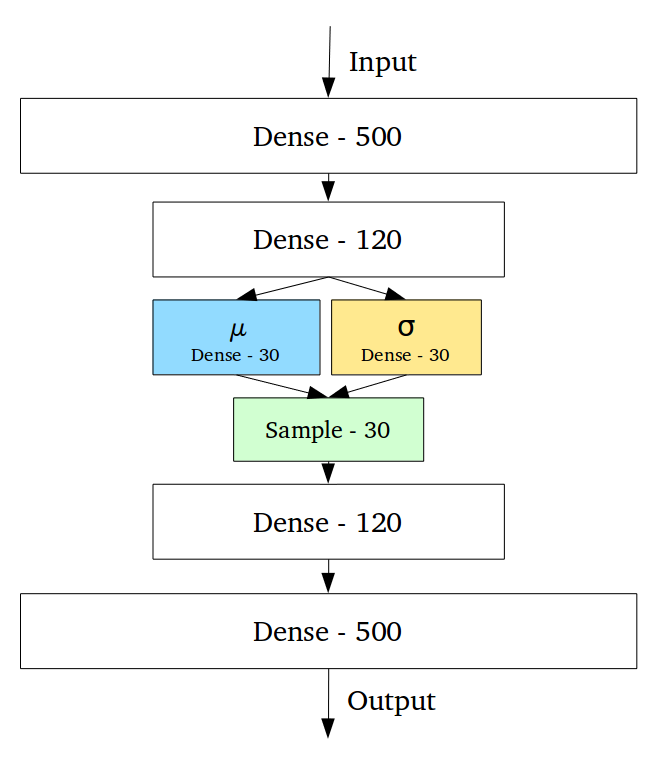
\includegraphics[scale=0.2]{./tex/encoder-decoder-network/varauto1.png}
    \caption{Architecture d'un Variationnal Autoencoder}
    \label{varauto1}
\end{figure}

\begin{figure}
    \centering
    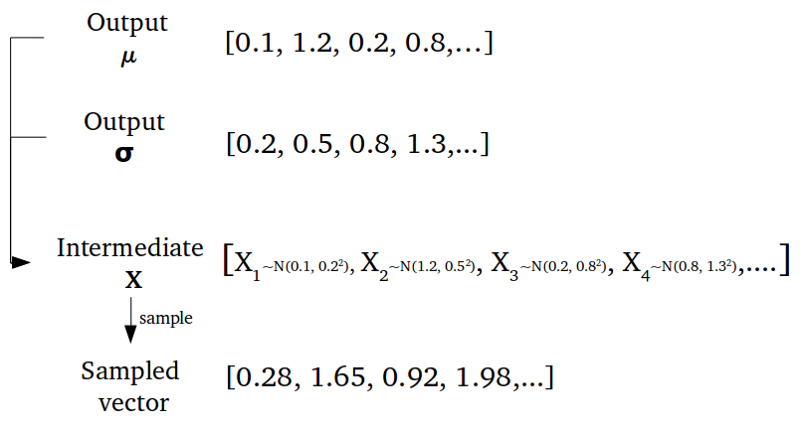
\includegraphics[scale=0.2]{./tex/encoder-decoder-network/varauto2.png}
    \caption{Détermination du vecteur de contexte par un Variationnal Autoencoder}
    \label{varauto2}
\end{figure}

\begin{figure}
    \centering
    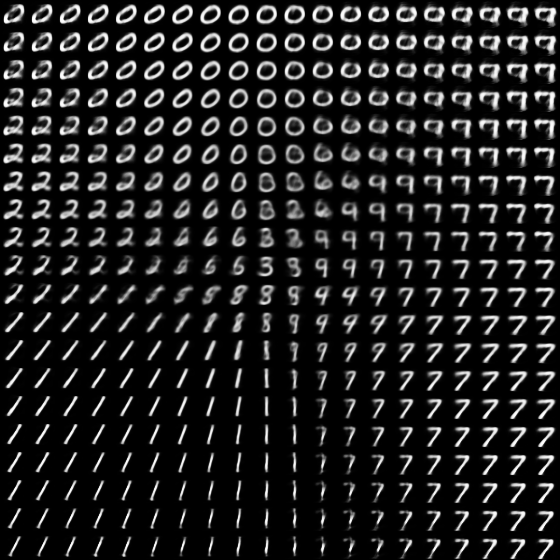
\includegraphics[scale=0.2]{./tex/encoder-decoder-network/varauto3.png}
    \caption{Generation d'image par un Variationnal Autoencoder entrainé sur MNIST}
    \label{varauto3}
\end{figure}
